\documentclass[luatex,mathserif,serif,utf8,table]{beamer}
\usetheme{moscow}
\usepackage{graphicx}
\usepackage{fontspec}
\setmainfont{Textbook New}
\usepackage{polyglossia}
\setotherlanguage{english}

\title{A data analysis competition}
\date{August~27,~2015}
\author{\underline{Nikita~Kazeev}\and Alexey~Rogozhnikov\and Andrey~Ustyuzhanin}
\institute{The Yandex School of Data Analysis}

\begin{document}
\frame{\titlepage}
\begin{frame}
  \frametitle{Physics - COMET}
  \begin{itemize}
  \item A planned experiment at J-PARC, Japan
  \item Searches for coherent neutrino-less conversion of a muon to an
    electron, $\mu^- + N(A,Z) \rightarrow e^- + N(A,Z)$.
  \item The process breaks the leptonic number conservation law.
  \item Previous upper limit was set by SINDRUM II in 2006, COMET is
    going to have 10000 times better sensitivity.
  \end{itemize}
\end{frame}

\begin{frame}
  \frametitle{Experiment idea} Smash muons into aluminum to make
  muonic atoms, see if any electrons fly out. 
  \newline \par Standard model, peak at 52.8 MeV:
  \begin{equation}
    \mu^{-} \rightarrow \nu_\mu + e^{-} + \overline{\nu}_e
  \end{equation}
  Charge lepton flavour violation, peak at 105 MeV:
  \begin{equation}
    \mu^{-}+\text{Al} \rightarrow e^{-} + \text{Al}
  \end{equation}
\end{frame}

\begin{frame}
  \frametitle{Detector}
  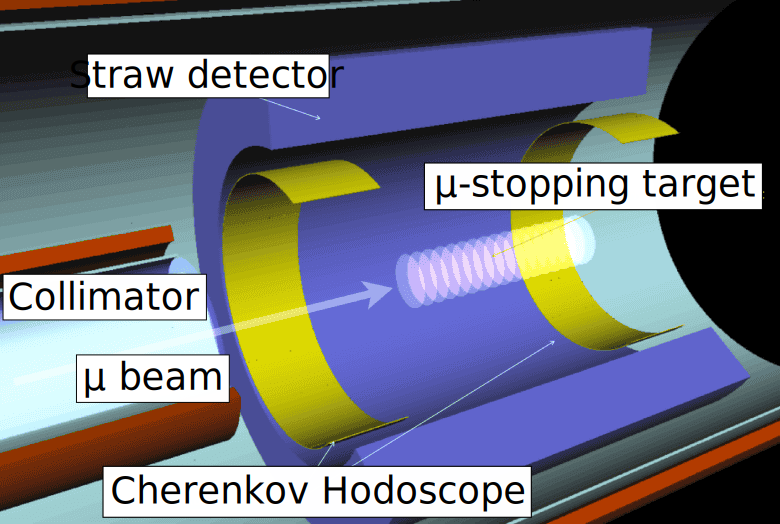
\includegraphics[width=\textwidth]{comet_3d_labels_imposed.pdf}
\end{frame}

\begin{frame}[c]
  \frametitle{Event}
  \begin{figure}
    \centering
    \includegraphics[height=0.9\textheight]{event.png}
  \end{figure}
\end{frame}

\begin{frame}
  \frametitle{Data}
  \begin{itemize}
  \item A Monte-Carlo simulation
  \item An event is a 'snapshot' of detector, it consists of data
    taken from all 4482 wires
  \item "energy" - energy deposited at the wire in GeV
  \item "relative\_time" - difference between time the straw tube
    detected energy and time of hodoscope in ns
  \item "label" - 0 for inactive wires, 1 for hits that are a part of
    a track, 2 for background hits
  \end{itemize}
\end{frame}

\begin{frame}
  \frametitle{Competition - basics}
  \begin{itemize}
  \item You are given some labeled data - train dataset
  \item You are given some unlabeled data - test dataset
  \item You are to predict the probability of being signal for hits from the test dataset
  \item You can work in team of two
  \item You are to receive a prize if you make into top-3 of your track
  \item You are to present your solution at the award ceremony - if you win
  \end{itemize}
\end{frame}

\begin{frame}
  \frametitle{Competition - technicalities}
  \begin{itemize}
  \item The link is in the StarterKit and the school website
  \item The test dataset is divided into two parts: public and private
  \item On the leaderboard you can view the score you get on the public part
  \item The final standings will be calculated on the private part
  \item The public/private split is based on individual hits, not events
  \item Private code sharing is not allowed - if you share, you must
    share with everybody via the forum
  \end{itemize}
\end{frame}

\begin{frame}
  \frametitle{Acknowledgments} We thank COMET collaboration (and
  specially Chen Wu) for allowing us to use this dataset, Ewen Gillies
  (ICL) for collaborating on the analysis it and Kaggle Inc. for
  hosting the competition.
\end{frame}

\end{document}